\documentclass[twocolumn, letterpaper, 10pt, twoside]{article}
%\usepackage[english]{babel} % English language/hyphenation
\usepackage{amsmath,amsfonts,amsthm} % Math packages
\usepackage[utf8]{inputenc}
\usepackage{graphicx}
\usepackage{caption}
\usepackage{subcaption}
\usepackage{pdfpages}
\usepackage{amssymb}
\usepackage{url}
\usepackage{tabu}
\usepackage{tikz} 
\usepackage{pgfplotstable}
\usepackage{pgfplots}
\usepackage{ragged2e}

\usepackage[hmarginratio=1:1,top=32mm,left=18mm,columnsep=20pt]{geometry} % Document margins

\usepackage{titlesec}
\usepackage{abstract}
\usepackage{booktabs} % Horizontal rules in tables
\usepackage{float} % Required for tables and figures in the multi-column environment - they need to be placed in specific locations with the [H] (e.g. \begin{table}[H])
\usepackage{paralist} % Used for the compactitem environment which makes bullet points with less space between them
\usepackage{enumitem} % \begin{itemize}[noitemsep]
\usepackage{parskip}
\setlength{\parindent}{3mm}
\setlength\tabcolsep{4pt}
\usepackage[labelsep=period]{caption}
\captionsetup[table]{name= \bfseries{TABLE}}
\renewcommand{\thetable}{\bfseries\Roman{table}}

%\newcommand{\horrule}[1]{\rule{\linewidth}{#1}} % Create horizontal rule command with 1 argument of height
\usepackage{fancyhdr} % Headers and footers
\pagestyle{fancy} % All pages have headers and footers
\fancyhead{} % Blank out the default header
%\fancyfoot{} % Blank out the default footer

\renewcommand{\thesection}{\Roman{section}} 
\renewcommand{\thesubsection}{\thesection.\Roman{subsection}}

\titleformat{\section}{\large\normalfont\bfseries\centering}{\thesection}{}{}
\titlespacing{\section}{0pt}{4pt}{0pt}
\titleformat{\subsection}{\normalsize\normalfont\it\bfseries\centering}{\thesubsection}{}{}
\titleformat{\subsubsection}{\small\normalfont\bf}{\thesubsection}{}{}

\renewcommand{\abstractname}{}    % clear the title
\renewcommand{\absnamepos}{empty} % originally center, stops loss of space
\newcommand{\comment}[1]{}
%----------------------------------------------------------------------------------------
%       My Commands
%----------------------------------------------------------------------------------------
%\renewcommand{\arraystretch}{1.2}
\makeatletter
\g@addto@macro\@floatboxreset\centering
\makeatother
%----------------------------------------------------------------------------------------
%----------------------------------------------------------------------------------------
\newcommand{\coursenum}{326}
\newcommand{\thetitle}{Experiment 32:\\Charge Oscillations and Energy Transfers in LRC Circuits} 

\rhead{Physics 326 \\ Experiment 32}
\lhead{Austin Beauchamp \\ V00825419 }
\rfoot{Department of Physics and Astronomy}
\lfoot{University of Victoria}
\renewcommand{\headrulewidth}{1pt}
\renewcommand{\footrulewidth}{1pt}
%\fancyfoot[LE,RO]{\thepage} % Custom footer text
%----------------------------------------------------------------------------------------
%       TITLE SECTION
%----------------------------------------------------------------------------------------
\title{\vspace{-10mm}\fontsize{15pt}{10pt}\selectfont\textbf{\thetitle}\vspace{-3mm}} % Article title
\author{
	\large
	{\textsc{Austin Beauchamp, University of Victoria}}\\[-7mm]}
\date{Submitted September 23rd, 2019}
%----------------------------------------------------------------------------------------

\begin{document}
	\twocolumn[
	\begin{@twocolumnfalse}
		\maketitle
		\thispagestyle{fancy} % All pages have headers and footers
		\vspace{-3mm}
		\begin{abstract}
			\section*{Abstract}
			
			This experiment aims to study the oscillatory properties of a circuit composed of an inductor, resistor, and capacitor: an LRC circuit. If too much charge builds up in the capacitor, electrostatic repulsion causes the current to switch directions, resulting in harmonic motion. There are three cases for discharge: overdamped, critically damped, and underdamped. Overdamped systems simply return to equilibrium at an aperiodic rate, critically damped systems return to equilibrium as fast as possible, and underdamped systems exhibit oscillatory behavior. For the underdamped system, we observe an oscillation frequency of $45.96$hz. This value proves inconsistent against two theoretical checks (ignoring and including circuit resistance) which could mainly be attributed to thermal drift of the probes.

     \end{abstract}
\vspace{7mm}
\end{@twocolumnfalse}
]

    \section*{I. Introduction}
 
 An LRC circuit consists of an inductor (L), resistor (R), and a capacitor (C) connected in series (figure 1). This creates a harmonic oscillator and has many applications in modern electronics in the form of signal filters. Forming an oscillator, and LRC circuit will have intrinsic wavelike properties, a resonant frequency and damping characteristics.  
 
 
 \begin{figure}[H]
 	\centering
 	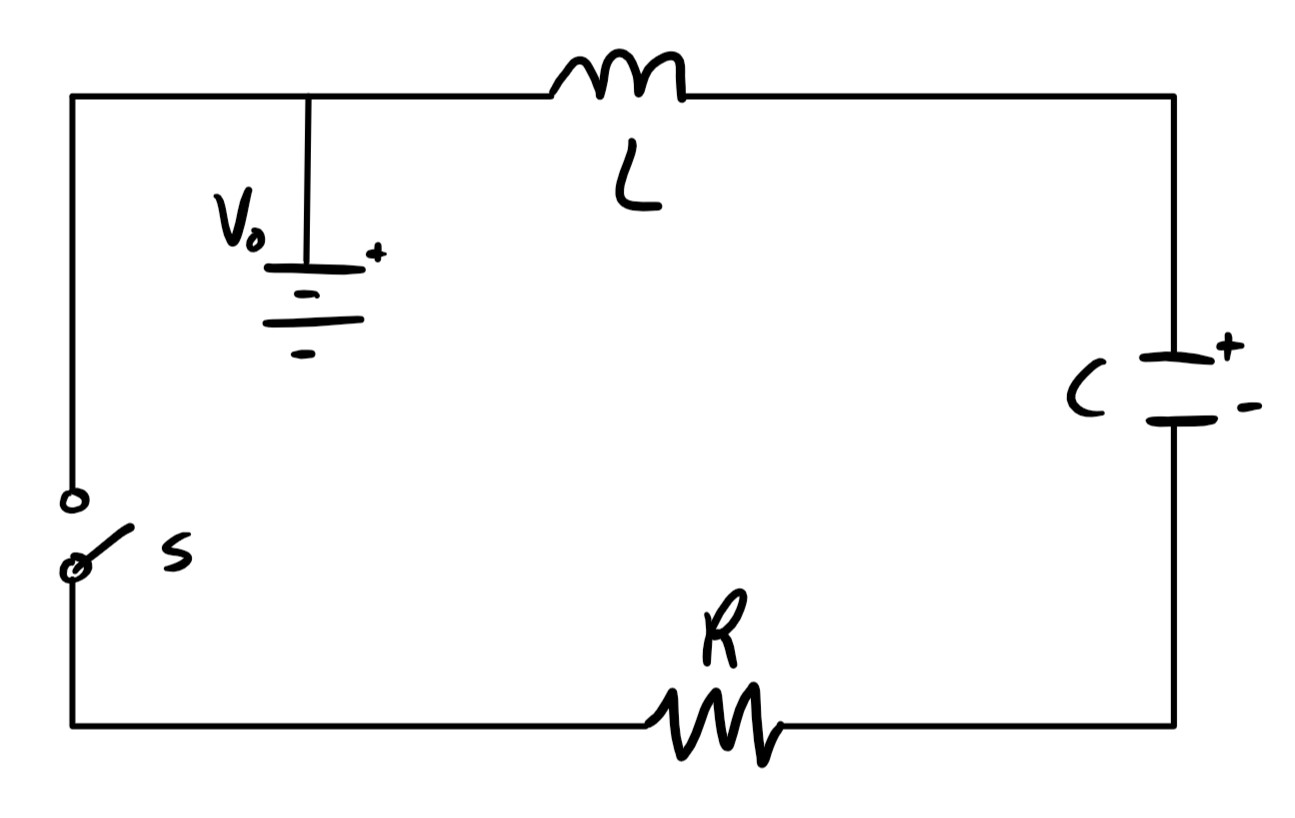
\includegraphics[width=.7\linewidth]{circuit.jpg}
 	\captionsetup{width=.8\linewidth,belowskip=-2mm,aboveskip=1mm}
 	\vspace{0.2cm}
 	\caption{\textbf{LRC Circuit} }
 \end{figure}

 Applying a voltage to the circuit results in a gradual response. The nature of the capacitor requires voltage buildup, so the reaction to the voltage takes time. The capacitors' energy storage in the electric field influences the inductors' magnetic field. As the capacitor continues to charge, electrostatic repulsion increases between charges in the capacitor. Eventually the repulsion because too large, causing a reverse in direction. This reversal in voltage direction creates the harmonic motion, and damping depends on the resistance of the entire circuit. Shorting the power supply allows the circuit to oscillate until all energy has been lost and the voltage returns to zero.
 
 
 For the circuit in figure 1, the total voltage is given by
 
  \begin{equation}
 V_o = L\frac{di}{dt} + iR + \frac{q}{C}
 \end{equation}
 
 where $q$ is the capacitor's charge and $i$ is the current. At the starting position $t_0 = 0$, the initial voltage $V_0 = 0$. Using $i = \frac{dq}{dt}$, the above equation transforms into 
 
 
 \begin{equation}
L\frac{d^2i}{dt^2} + R\frac{di}{dt} + \frac{i}{C} = 0
 \end{equation}  
 
 
 Assuming the differential equation's solution takes the form $i = Ae^{st}$:
 
   \begin{equation}
Ae^{st}(Ls^2 + Rs + \frac{1}{C}) = 0 
 \end{equation}
 
 Due to $Ae^{st}$ never equaling zero, we take $(Ls^2 + Rs + \frac{1}{C}) = 0 $. Solving for $s$,
 
  \begin{equation}
s = -\frac{R}{2L} \pm \sqrt{\frac{R^2}{4L^2} - \frac{1}{LC}}
 \end{equation}
 
 This results in $s$ having two values: $s_1$ and $s_2$. The final solution to the differential equation (2):
 
   \begin{equation}
i = Ae^{s_1t} + Be^{s_2t}
 \end{equation}
 
 Because the radical in (4) can be real-valued, complex, or zero, we have three separate cases for damping. 
 
 Where A and B are two arbitrary constants that are determined by the initial conditions. There are three possible solutions for equation (5) depending on whether the value under the square root is positive, zero, or negative. These solutions are: 
 
 \textbf{{Case 1:} Overdamping}
 
\begin{equation}
(\frac{R}{2L})^2 - \frac{1}{LC} > 0 
\end{equation}

A real-valued radical, resulting in aperiodic discharge of the capacitor. Both $s_1$ and $s_2$ are real valued and the solution can be written as

   \begin{equation}
i = e^{-\frac{R}{2L}t}(Ae^{\omega t} + Be^{-\omega t})
\end{equation}

where

   \begin{equation}
\omega = \sqrt{\frac{R^2}{4L^2} - \frac{1}{LC}}
\end{equation}
  
  Substituting the initial condition $i = 0$ into (7), we have $B = -A$. Writing (7):
  
 \begin{equation}
  i = Ae^{-\frac{R}{2L}t}(e^{\omega t} - e^{-\omega t})
 \end{equation}
  
  Determining $A$ requires a boundary condition on $\frac{di}{dt}$, which we define as $i$ being in a positive clockwise direction. After differentiating and substituting in $L\frac{di}{dt} = -V_0$ at $t_0 = 0$, we find that $A = -\frac{V_0}{2\omega L}$, for a final equation 
  
  \begin{equation}
  i = -\frac{V_0}{2\omega L}e^{-\frac{R}{2L}t}(e^{\omega t} - e^{-\omega t})
  \end{equation}
  
  Both terms in  (10) decay at different rates, resulting in the aperiodic decay.
  
\textbf{{Case 2:} Critical Damping}

\begin{equation}
(\frac{R}{2L})^2 = \frac{1}{LC}
\end{equation}

The special case where $S_1$ and $S_2$ are equal. The discharge across the capacitor is still aperiodic, however this case reaches equilibrium the fastest. The solution takes the form

   \begin{equation}
i = e^{-\frac{R}{2L}t}(A + Bt) 
\end{equation}
with ($\omega = 0$).
By the superposition principle, the two solutions $i = Ae^{-\frac{R}{2L}t}$ and $i = Bte^{-\frac{R}{2L}t}$ summed are also a solution:

\begin{equation}
i = \frac{-V_o}{L}te^{-\frac{R}{2L}t}
\end{equation}
Where $-V_0$ is the emf applied by the capacitor at time $t_0 = 0$.

The voltage across the inductor is 

\begin{equation}
v_L = V_0 (1-\frac{R}{2l}t)e^{-\frac{R}{2L}t}
\end{equation}

and the voltage across the capacitor is 

\begin{equation}
v_C = V_0 (1+\frac{R}{2l}t)e^{-\frac{R}{2L}t}
\end{equation}

and the voltage across the resistor is

\begin{equation}
v_R = i * R_{resistor} = \frac{-V_0}{L}te^{-\frac{R}{2L}t}R_{resistor}
\end{equation}

\textbf{{Case 3:} Underdamping}

   \begin{equation}
(\frac{R}{2L})^2 < \frac{1}{LC}
\end{equation}

Here $s_1$ and $s_2$ are complex, with the solution becoming:

   \begin{equation}
i = e^{-\frac{R}{2L}t}(Ae^{j\omega t} + Be^{-j\omega t})
\end{equation}
	
Following similar steps from case 1, the solution for current is given by

\begin{equation}
i = \frac{-V_0}{\omega L}e^{-\frac{R}{2L}t}sin(\omega t)
\end{equation}	

This equation represents a sine function which exponentially decreases in amplitude. The natural angular frequency is $\omega$, and the natural frequency is 

\begin{equation}
f = \frac{1}{2\pi}\sqrt{\frac{1}{LC}}
\end{equation}

The energy dissipated as heat in the resistor over an interval $\Delta t$ is given by 

\begin{equation}
	\int_{t_n}^{t_{max}}Ri^2dq \approx R(I^2)_{AV} \Delta t
\end{equation}

where $(I^2)_{AV} = \frac{I_{tn^2} + I_{t_{n+1}}}{2}$

The inductor and capacitor energy amounts at a given time are defined by

\begin{equation}
E_L = \frac{1}{2} L (\frac{v_R}{R_{resistor}})^2
\end{equation}

and 

\begin{equation}
E_C = \frac{1}{2} Cv_C^2
\end{equation}


 \section*{II. Apparatus}
    The apparatus (figure 2): inductor, capacitor, resistance box, power supply, LabPro with differential probes and computer. 
    
    \begin{figure}[H]
   	\centering
   	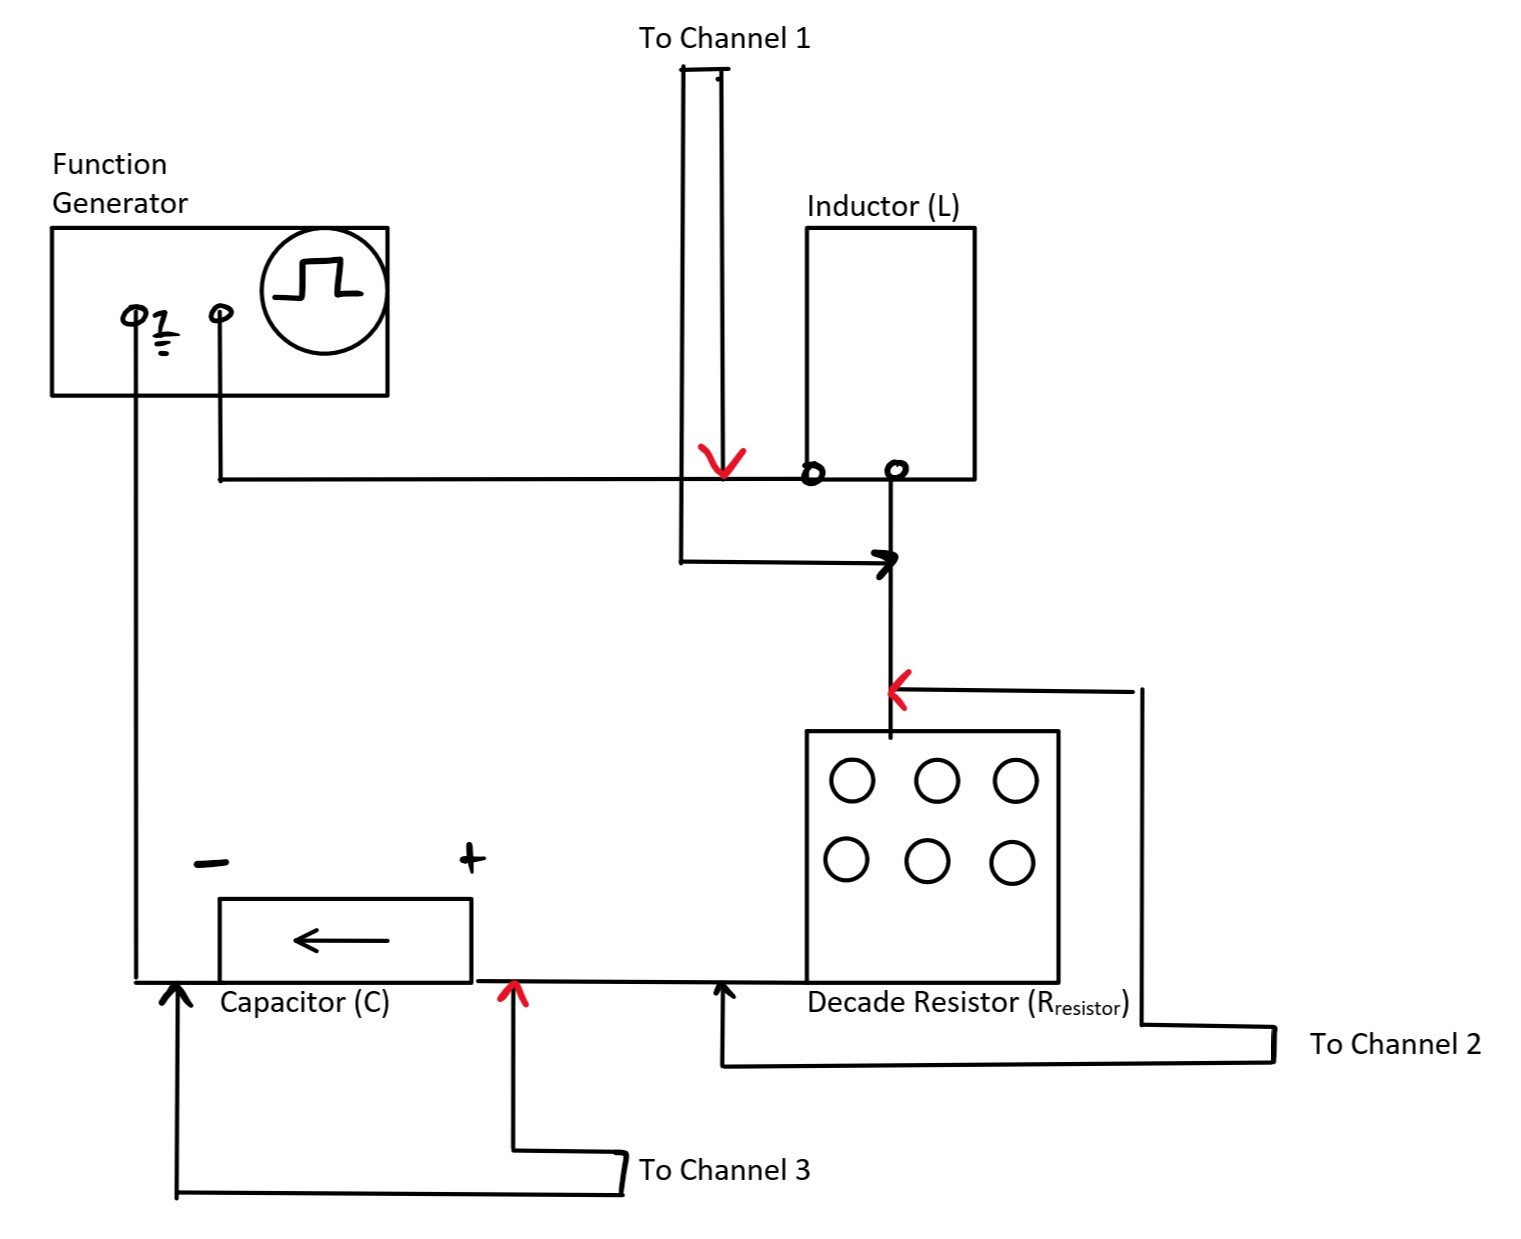
\includegraphics[width=.7\linewidth]{apparatus.jpg}
   	\captionsetup{width=.8\linewidth,belowskip=-2mm,aboveskip=1mm}
   	\vspace{0.2cm}
   	\caption{\textbf{Diagram of Apparatus} Input clips shown in red, reference clips are black arrows.}
   \end{figure}
   
 \section*{III. Procedure}
      
	\indent Initial setup included measuring the inductor's inductance and resistance, and the capacitors capacitance, shown in table 1. The function was connected directly to the voltage probes to measure the output signal. A square waveform of about 5Hz, with minimum at 0V and maximum at 4V was created. Before connecting the circuit as in figure 2, the probes were all shorted and zeroed before each case was observed. A negative trigger voltage on the inductor provides an unambiguous starting point for data collection.
	
	\begin{table} [H] 
		\centering
		\tabulinesep=1.5mm
		\begin{tabu} { | X[c] | X[c] | }
			\hline \centering
			$R_{Fuction Generator}$, R & (50 $\pm$ 0.1) $\Omega$ \\
			\centering
			$R_{Inductor}$, R & (110.0 $\pm$ 0.1) $\Omega$ \\
			\centering
			Inductor, L & (1.036 $\pm$ 0.001) H \\
			\centering
			Capacitor, C & (10.1 $\pm$ 0.01) $\mu$F \\
			\hline
		\end{tabu}
		\captionsetup{width=.8\linewidth}
		\vspace{-1mm}
		\caption{Circuit component values.}
	\end{table}
	
	\textbf{{Case 1:} Overdamping}
	Overdamping, also called normal damping, was created by selecting a resistance value greater than the critical damping resistance value. The critical resistance was calculated using $L = 1.036 \pm 0.1\% $ and $C = (10.1 \pm 0.1\%)$
	
	\begin{equation*}
	R_{critical} = 2 \sqrt{\frac{L}{C}} =(641 \pm .14\%) \Omega
	\end{equation*}
	
	The resistance box was set to $1k\Omega$ to ensure normal damping. The resistance across the capacitor is plotted in figure 3, where we see a decay from 4V to 0V.
	
	\textbf{{Case 2:} Critical Damping}
	The previous calculation for critical damping is for the entire circuits resistance. Finding the value for the resistor: 
	
	\begin{equation*}
	R_{resistor} = R_{critical} - R_L - R_FG 
	\end{equation*}
	\begin{equation*}
	= (641 \pm .14\%)\Omega - (110.0 \pm 0.1\%)\Omega - (50 \pm 0.2\%)\Omega 
	\end{equation*}
	\begin{equation*}
	= (481 \pm 0.26\%)\Omega
	\end{equation*}
	
	The voltage curves across the capacitor and the resistor are plotted in figure 4, along with their theoretical curves from equation (15) and (16). Compared to the normal damped system in figure 3, the voltage very clearly discharges to zero across the capacitor quicker in the critically damped system. Both of the experimental curves also follow closely to their theoretical counterparts, suggesting correct results. 
	
	The energies of the system were analyzed and plotted in figure 5. The system includes energies across the inductor, $E_L$, and capacitor, $E_C$ (equations 14 and 15, respectively), the total energy $E_T = E_L + E_C$, the summation of heat dissipated by the resistor, $E_HT$, (equation 21), and the conservative energy, $E_{conservative}$. The initial discharge from the capacitor appears to increase the energy of the inductor, which eventually both decay to zero. $E_T$ and $E_HT$ are inversely proportional. The energy of the circuit gets lost as heat energy in the resistor, resulting in the curves being inversely proportional. The initial energy in the system is constant, resulting in the $E_{conservative}$ curve staying relatively constant (the system includes the circuit and heat loss in the resistor). 
	
			
	\textbf{{Case 3:} Underdamping}
	
	For the final case, a resistor value of $14\Omega$ was chosen for the resistor, creating an underdamped system. The resistance across all three circuit components is plotted in figure 6. An oscillatory pattern appears across all three components, with the inductor and capacitor appearing exactly opposite in amplitude and the resistor with a much smaller oscillation (however still existent). 
	
	Measuring the frequency of oscillation across the capacitors voltage:
	
	\begin{equation*}
	T =  T_1 - T_2 = 0.021758
	f = \frac{1}{T} = 45.96 Hz
	\end{equation*}
	
	The theoretical frequency (ignoring circuit resistance):
	
	\begin{equation*}
	f = \frac{1}{2\pi}\sqrt{\frac{1}{LC}}
	\end{equation*}
	\begin{equation*}
	= \frac{1}{2\pi}\sqrt{\frac{1}{(1.036H \pm 0.1\%)(10.1\mu F \pm 0.1\%)}} 
	\end{equation*}
	\begin{equation*}
	= (49.2 \pm 0.14\%)
	\end{equation*}
	
	Performing a consistency check:
	
	\begin{equation*}
	|f_{experimental} - f_{theo}| \stackrel{?}{\leq} \Delta f_{experimental} + f_{theo}
	\end{equation*}
	\begin{equation*}
	|46.0 Hz - 49.2Hz | \stackrel{?}{\leq} 0.07 Hz
	\end{equation*}
	\begin{equation*}
	3.2Hz \nleq 0.07Hz
	\end{equation*}
	
	The values are inconsistent. Not ignoring te total circuit resistance:
 
 	\begin{equation*}
	 f = \frac{1}{2\pi}\sqrt{\frac{1}{LC} - \frac{R^2}{4L^2}}
	\end{equation*}
 	
 	\begin{equation*}
	f = \frac{1}{2\pi}
	\end{equation*}
	\begin{equation*}
	\sqrt{\frac{1}{(1.036H \pm 0.1\%)(10.1\mu F \pm 0.1\%)} -
		\frac{(175 \pm 0.57\%)^2}{4*(1.036 \pm 0.1\%)^2}}
	\end{equation*}
	\begin{equation*}
	= 47.3Hz \pm 0.3\%
	\end{equation*}
	\begin{equation*}
	= (47.3 \pm 0.14)Hz
	\end{equation*}
	
 	Performing a consistency check:
 
	 \begin{equation*}
	 |f_{experimental} - f_{theo}| \stackrel{?}{\leq} \Delta f_{experimental} + f_{theo}
	 \end{equation*}
	 \begin{equation*}
	 |47.3 Hz - 49.2Hz | \stackrel{?}{\leq} 0.14 Hz
	 \end{equation*}
	 \begin{equation*}
	 1.9Hz \nleq 0.14Hz
	 \end{equation*}
 
 	These values are inconsistent, however they are closer to consistent than when ignoring circuit resistance. Possible sources of error resulting in inconsistencies includes thermal drift of the probes. Although the probes were zeroed, it is possible that thermal drift caused their readings to not be truly centered at zero.
 	
 	The same energy analysis for case 2 was done for case 3, plotted on figure 7. $E_C$ and $E_L$ appear to have an inversely proportional relationship, where the capacitors energy decreases causes the inductors energy to increase. We see these curves oscillate after reaching zero, instead of remaining there like in case 2. The curves for $E_T$ and $E_HT$ are also inversely proportional as expected, with plateaus occurring when the capacitor peaks during its oscillatory cycle. This is due to the charge/discharge of the capacitor not being instantaneous, and the capacitor storing its energy while the circuit reverses. Disregarding initial noise, the $E_Conservative$ line remains relatively consistent, however there is a slight downwards slope as it coincides with $E_HT$ curve. This suggests another form of energy loss other than heat through the resistor. Accelerating charged particles are known to emit energy in the form of electromagnetic waves. During an oscillatory cycle, electrons will physically have to accelerate to switch directions, losing energy in the process.


\comment{
\begin{table} [H] 
	\centering
	\tabulinesep=1.3mm
	\begin{tabu} { | X[c] | X[c] | X[c] |}
		\hline \centering
		\textbf{Case} & \textbf{$R_{Resistor}$} & \textbf{R} \\
		\hline \centering
		1 & 1111.98 $\pm$ 2.08 & 1250.48 $\pm$ 1.88 \\
		\centering
		2 & 486.74 $\pm$ 2.08 & 625.24 $\pm$ 1.88 \\
		\centering
		3 & 153.5 $\pm$ 0.2 & 15 \\
		\hline
	\end{tabu}
	\captionsetup{width=.8\linewidth}
	\vspace{-1mm}
	\caption{All values are in units of $\Omega$. $R_{Resistor}$ is obtained through the equation introduced in the procedure,  $R_{resistor} = R - R_L - R_{FG}$. R is obtained from equation (\textbf{32.6}) for cases 1 and 2, and given in the procedure for case 3.}
	
\end{table}
}


\section*{IV. Conclusion}
We studied the properties of harmonic oscillation in an LRC circuit, examining overdamping, underdamping, and critical damping. Critical damping occurred with a total circuit resistance value of $(641 \pm .14\%) \Omega$, and showed that the system discharged to equilibrium quicker than over and underdamped systems. The oscillatory period was experimentally determined to $45.96$hz, but was inconsistent with theoretical values when ignoring and including circuit resistance; however, including circuit resistance in the calculations brought the experimental and theoretical values closer together. The main source of error is most likely thermal drift in the probes. The experiment also approximately demonstrated conservation of energy, with slight loss due to accelerating charged particles losing energy during a current direction switch.
   

\end{document}